% !TEX root = ../rawlik-phd-thesis.tex
\chapter{Coil design}
\label{ch:coil_design}

In this chapter a new method to design a coil producing an arbitrarily shaped magnetic field is introduced. In this method the path of the coil's wires are restricted to a regular grid, the solution is then found by a simple least squares minimum. Practical applications, in particular in an active magnetic shielding, are discussed.




\section{Introduction}
\marginpar{This chapter is largely adapted from the author's publication CITE WHEN AVAILABLE}
How can we design a coil, or more generally, an arrangement of wires, to produce a desired magnetic field? In its simplest form this is a textbook problem (e.g.\ ex. 6.55 and 6.62 in Ref.\,\cite{Purcell}).
Yet in general it is surprisingly hard, and the solutions (how the wires making up the coils should be laid) complicated.
The most widespread application of high-performance coils is in Magnetic Resonance Imaging (MRI), where gradient coils give the possibility to produce spatial images.
In the 1980s elaborate methods of MRI coil design had already been developed.
These methods range from optimizing positions of discrete windings, where the use is made of symmetries specific to MRI, to analytical methods yielding surface current density, which is then discretised.
A general overview can be found in Ref.\,\cite{Turner1993}.
Another field known for complex, precise coils is plasma confinement, in particular stellarators~\cite{Beidler1990}. There analytical solutions for the surface current density find their use, too.

Here, a new method is presented that may not be competitive in terms of precision, but is distinct in its simplicity---also when it comes to construction of the designs. The procedure relies on an algebraic representation of the problem, where coil design is simplified to a simple linear least squares problem.
In the method the coils are restricted to a user-defined mesh, resulting in easy to deal with spatial constraints.

The discussion is based on textbook linear algebra techniques, notably solving an over-determined system of linear equations, thoroughly discussed e.g.\ in Ref.\,\cite{Anton}.
The main physics problem, calculating the magnetic field of coils composed of straight wire segments, is briefly discussed here.
More in-depth discussions can be found, for example, in Ref.\,\cite{Griffith}.
Furthermore, the implementation of the discussed problems, including examples, has been published and open-sourced~\cite{Coilsjlcode}.

We begin with a description of our model for a restricted two-dimensional case and generalize it to three dimensions. We then present how the model is used to design a coil, based on an example. Further we discuss possibilities of simplifying the solution. Another section is devoted to practical considerations, significant for the eventual construction. Finally, the application to active magnetic field shielding is considered.




\section{Coils as a linear space}
Consider all the possible coils that can be constructed by laying a wire on a surface of a square. The possibilities are endless.
More precisely, as the wires are shifted by arbitrarily small distances, overlapping and crossing other wires, the problem has an infinite number of degrees of freedom.
Here, an algebraic representation that reduces the number of degrees of freedom to just a few is proposed.

We start with a straight, finite wire segment spanned between points $\mathbf{x}_1$ and $\mathbf{x}_2$ (represented by vectors in an arbitrary coordinate system) and carrying current $I$, as depicted in Fig.\,\ref{fig:biot-savart}. The magnetic field it produces in the point $\mathbf{p}$ can be calculated with the use of the Biot-Savart law. Consider the vector normal to the wire through the point $\mathbf{p}$:
\begin{equation}
  \boldsymbol{\uprho} = (\mathbf{x}_1 - \mathbf{p}) - \left( \left( \mathbf{x}_1 - \mathbf{p} \right) \cdot \mathbf{n} \right)\mathbf{n} \ ,
\end{equation}
where $\mathbf{n}$ is a unit vector in the direction $\mathbf{x}_2 -\mathbf{x}_1$.
The magnitude of the magnetic field at point $\mathbf{p}$ is then~\cite{Griffith}:
\begin{equation}
  \label{eq:biot_savart}
  B = \frac{\mu_0 I}{4 \pi \rho} \, \left| \sin \alpha_2 + s\, \sin \alpha_1 \right| \ ,
\end{equation}
where the angles $\alpha_i$ are not directed
\begin{equation}
  \sin \alpha_i = \frac{ \left\lVert \left( \mathbf{x}_i - \mathbf{p} \right) \times \boldsymbol{\uprho} \right\rVert }{ (x_i  - p) \rho } \ .
\end{equation}
$s$ is $+1$ if $\boldsymbol{\uprho}$ points onto the wire segment (between points $\mathbf{x}_1$ and $\mathbf{x}_2$) and $-1$ otherwise:
\begin{equation}
  s = \mathrm{sgn}\left( \tfrac{1}{2} \left\lVert \mathbf{x}_2 - \mathbf{x}_1 \right\rVert -
  \left\lVert \mathbf{p} + \boldsymbol{\uprho} - \tfrac{1}{2} \left( \mathbf{x}_1 + \mathbf{x}_2 \right) \right\rVert \right) \ .
\end{equation}
\marginpar{Another formulation, with better numerical properties close to the axis of the wire, can be found in Ref.\,\cite{Hanson2002}.}
The direction of the field is given by the right-hand principle
\begin{equation}
  \mathbf{B} = \frac{B}{\rho} \boldsymbol{\uprho} \times \mathbf{n} \ .
\end{equation}
This formulation is independent of the coordinate system (coordinate-system dependent solutions can be found e.g.\ in Ref.\,\cite{Grivich2000}).

\begin{figure}
  \centering
  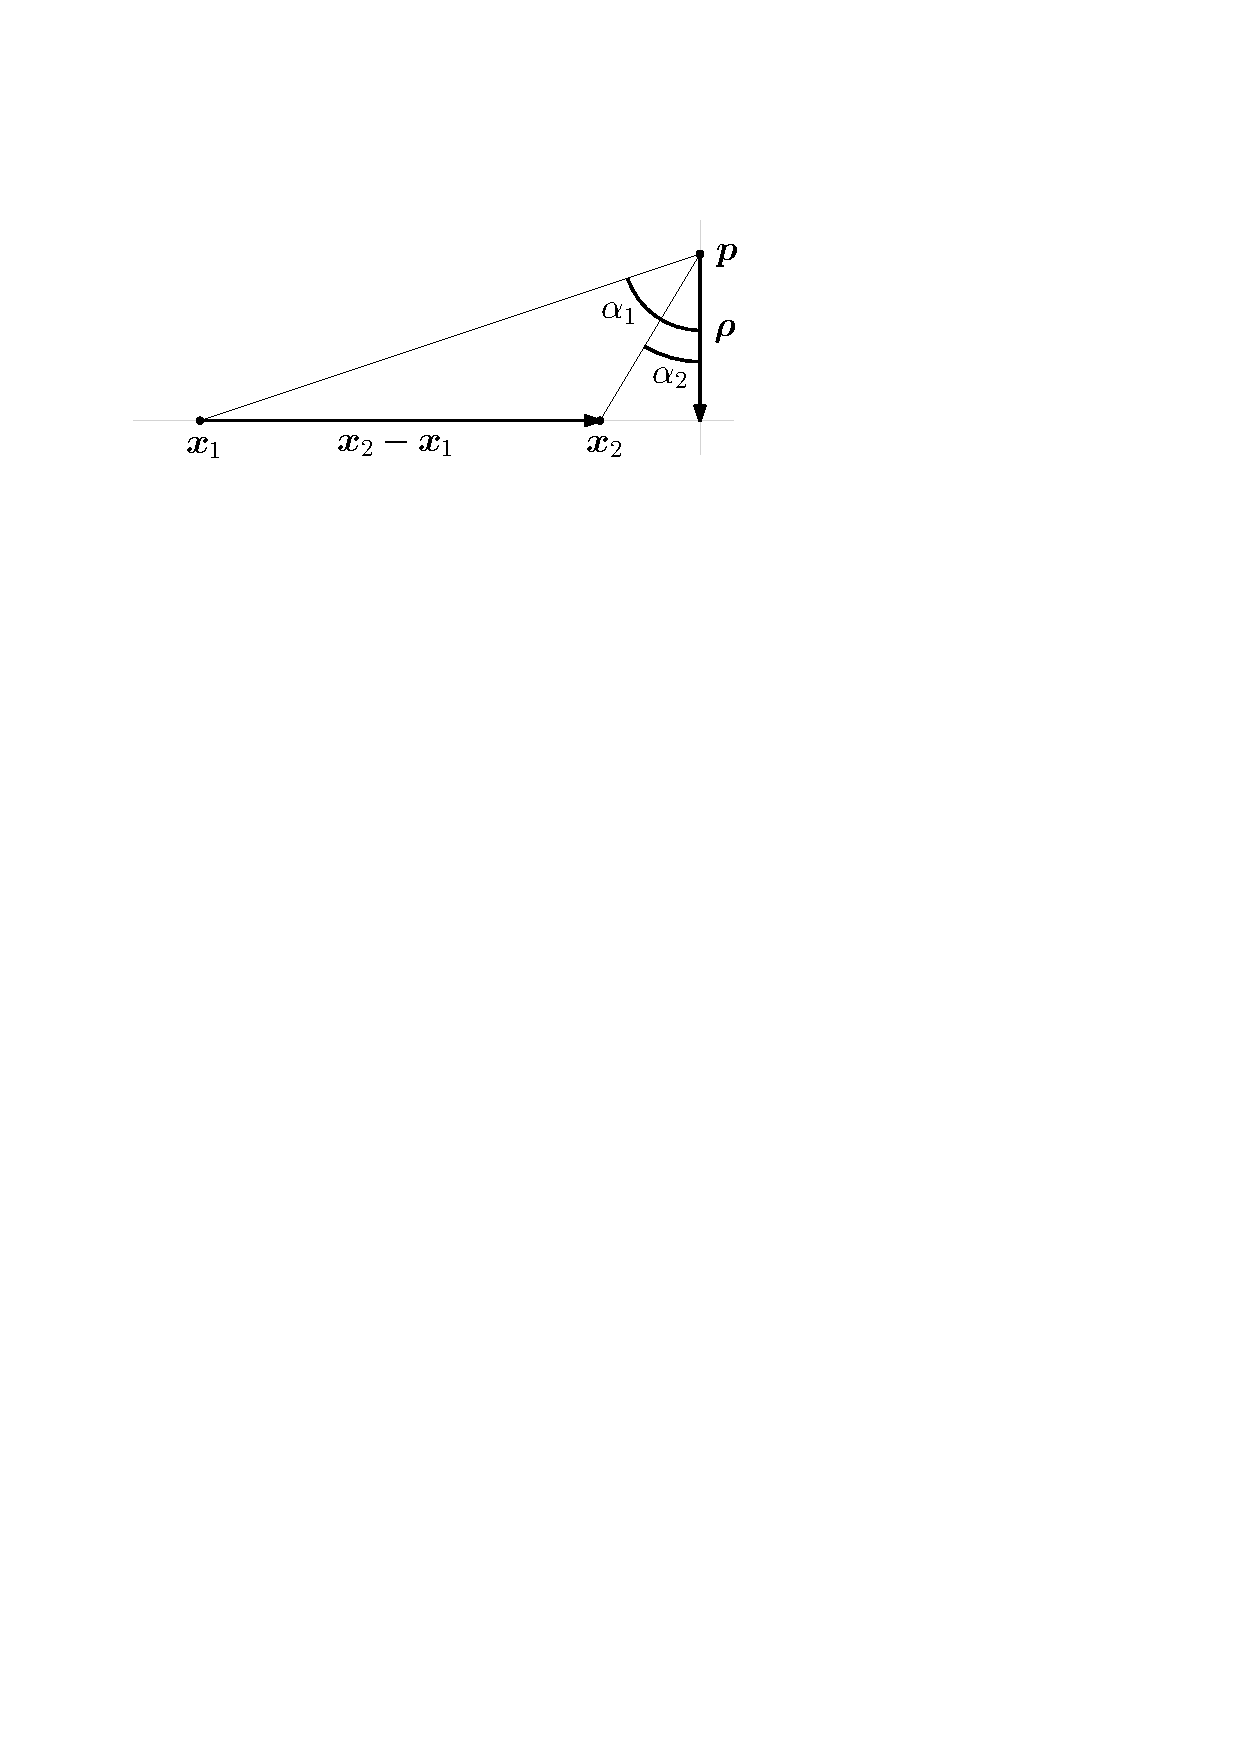
\includegraphics[width=0.6\linewidth]{gfx/coils/biot_savart.pdf}
  \caption{The setting for calculating the magnetic field produced in point $\mathbf{p}$ by a straight wire segment from $\mathbf{x}_1$ to $\mathbf{x}_2$.}\label{fig:biot-savart}
\end{figure}

Imagine four wire segments making up a square loop---a coil.
It produces a certain magnetic field in the entire space $\mathbf{B}(\mathbf{x})$ following the superposition principle, by summing the fields produced by each segment of the coil.
When the current in the coil is changed only one parameter of the magnetic field is altered---the magnitude, but not its shape.
Therefore, it can be said that one coil spans a one-dimensional space of magnetic fields it can produce.
Adding a second coil creates a system spanning a two-dimensional space of fields, as the magnetic field is additive. Going a step further, four square coils tiled to form a larger square form a four-dimensional space, as shown in Fig.\,\ref{fig:coils_tile_basis}.
Any coil restricted to a $2 \times 2$ grid can be represented in the base of the four tile-coils.

The range of magnetic fields reachable by coils restricted to a grid is a subset of all possible fields that can be created with coils constructed on the square's surface. The size of the subset is controlled by $N$, the number of tile-coils forming the grid.
In this system a coil is fully described by a vector of $N$ currents, one in each of the tile-coils denoted by $\mathbb{I}$. The problem of coil design is thereby simplified to finding a vector $\mathbb{I}$.

\begin{figure}
  \centering
  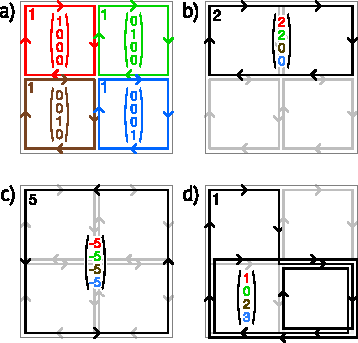
\includegraphics[width=0.6\linewidth]{gfx/coils/tile_basis.pdf}
  \caption{a) A basis of four tile coils on a flat square. Any coil which has its wires restricted to lie on the $2 \times 2$ grid can be represented as a linear combination of the four base tile coils. b, c, d) Three coils are presented together with their explicit coordinates in the basis.}\label{fig:coils_tile_basis}
\end{figure}

Generalisation onto a cube is simple.
A cube is made up of six square faces. Interestingly, for the assembly in the three-dimensional space one degree of freedom is lost.
Figure~\ref{fig:coils_tile_kernel} illustrates the simplest case where $N = 6$, a configuration in which finite currents in all six coils cancel and no magnetic field is produced.
Such a combination of currents can be added to any solution with no effect on the produced field.
Effectively, the space of the fields they can produce has dimension five (i.e.\ $N-1$).
In other words, the mapping of $\mathbb{I}$ onto fields $\mathbf{B}(\mathbf{x})$ has in this case a one-dimensional kernel.
This fact is of importance when it comes to numerically solving the system.

\begin{figure}
  \centering
  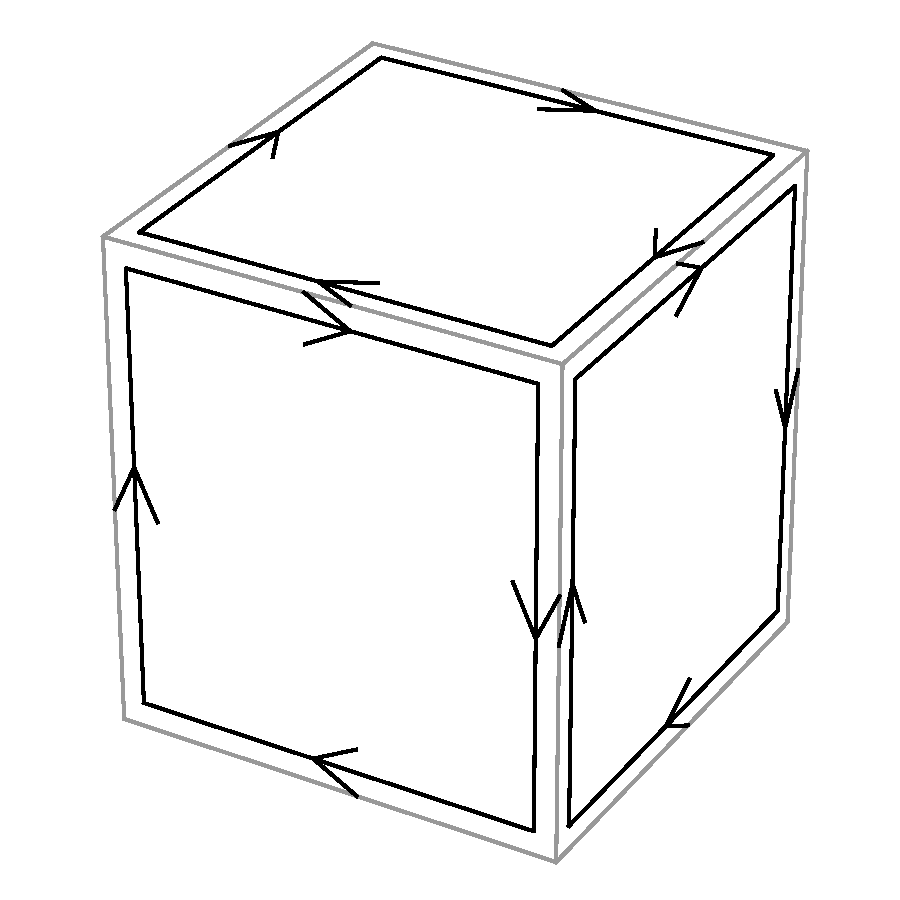
\includegraphics[width=0.5\linewidth]{gfx/coils/tile_kernel2.pdf}
  \caption{An arrangement of $N = 6$ tile coils on a cube which produces no magnetic field. The currents in the tiles are equal and flow in the directions as indicated. The currents on the invisible faces are analogous to the ones seen in front. For clarity, the coils are depicted slightly smaller. In the model the currents are identical with the edges of the cube.}\label{fig:coils_tile_kernel}
\end{figure}

This is the foundation of the method. The restriction to a grid on a cuboid enables all coils in the restricted space to be described by a vector of $N$ numbers.




\section{Coil design}
In the problem of coil design a coil or an arrangement of coils is sought, which best approximates a given field in a certain volume. The volume we shall call \emph{the volume of interest}. Rather than considering the whole volume, an ensemble of $m$ points of interest on its surface is selected (the surface is sufficient because $\nabla \cdot \mathbf{B} = 0$). Henceforth, only the magnetic field $\mathbf{B}(\mathbf{x})$ at these points is considered. The values $\mathbf{B}(\mathbf{x}_i)$ for $i = 1 .. m$ are gathered into a vector of dimension $3m$ ($B_x$, $B_y$ and $B_z$ in each point), which we shall denote $\mathbb{B}$.

As mentioned before, the magnetic field produced by a coil at any given point in space is proportional to the current in this coil.
With many coils present it is a linear combination of the currents of all coils in the system.
In absence of an external magnetic field the system of $N$ tiles and $m$ points of interest is thus described by a simple linear equation
\begin{equation}
  \label{eq:matrix}
  \mathbb{B} = M \, \mathbb{I}\ ,
\end{equation}
where $M \in \mathbb{R}^{3 m} \times \mathbb{R}^{N}$ is a matrix of proportionality constants.
For example, the element $M_{(5, 2)}$ is the proportionality constant between the current in the second of $N$ coils and the magnetic field in the $y$ direction in the second of $m$ points of interest, $B_y(\mathbf{x}_2)$.
The matrix $M$ can be calculated analytically using the Biot-Savart law.

Equation~\ref{eq:matrix} with $3m > N - 1$ is an over-determined system of linear equations, $\mathbb{I}$ being the vector of unknowns.
The optimal least-squares solution $\mathbb{I}_0$ to produce $\mathbf{B}_0(\mathbf{x})$ in the volume of interest is
\begin{equation}
  \label{eq:requirement}
  % M \, \mathbb{I} \stackrel{!}{=} \mathbb{B}_0
  \mathbb{I}_0 = \arg\,\min_{\mathbb{I}} {\left( M \mathbb{I} - \mathbb{B}_0 \right)}^2 \ .
\end{equation}
The optimal solution can be calculated with the normal equation~\cite{Anton}:
\begin{equation}
  \mathbb{I}_0 = {\left( M^\mathrm{T} M \right)}^{-1} M^\mathrm{T} \mathbb{B}_0 \ ,
\end{equation}
\marginpar{Least-squares is solved with a backslash operator in MATLAB-like languages:\\
\texttt{I0 = M \textbackslash{} B0.}}
but the problem is typically solved numerically.
The majority of numerical software packages use the QR decomposition (a product of an orthogonal and upper-triangular matrix) of the matrix $M$, which is more numerically stable when compared to the normal equation.

Depending on the properties of $M$ the optimum may be multidimensional.
As already mentioned, an arrangement of coils on a cube has a one-dimensional kernel, which will always cause the optimum to be at least one-dimensional.
In these cases, we will call $\mathbb{I}_0$ the unique least-norm solution, which minimizes the total current in the system.
$\mathbb{I}_0$ is the vector of the optimal currents in the tile arrangement of coils for approximating $\mathbf{B}_0(\mathbf{x})$ in the volume of interest.

\begin{figure}
  \centering
  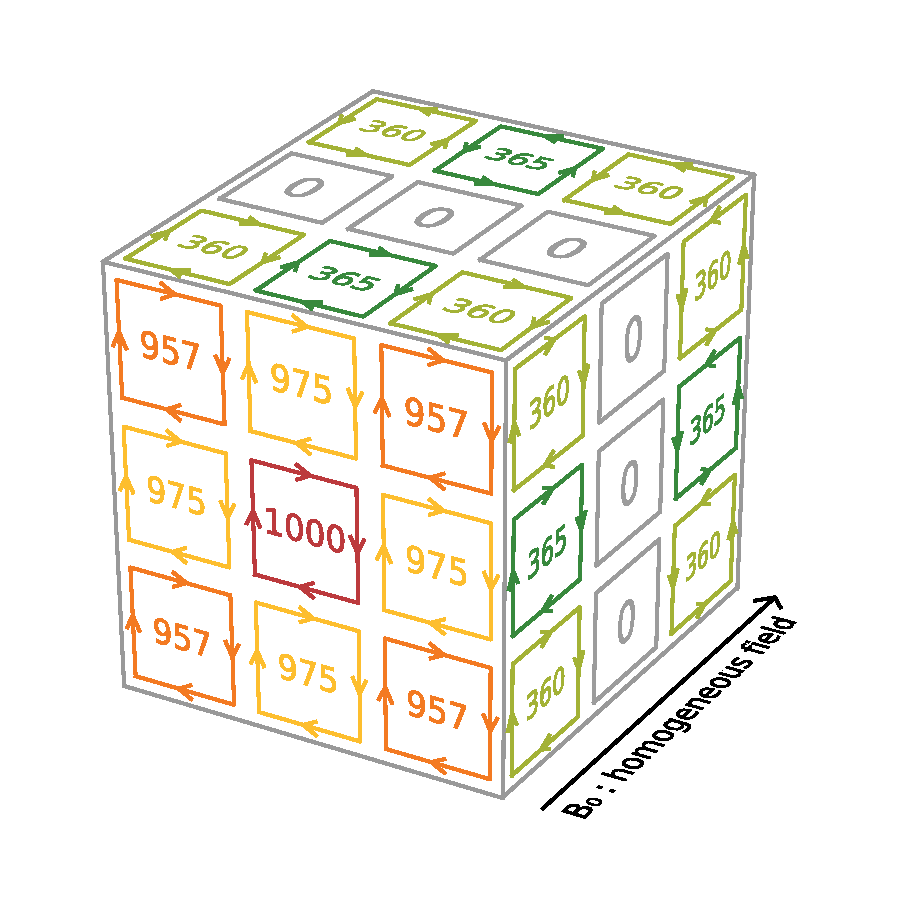
\includegraphics[width=\linewidth]{gfx/coils/homogeneous_tiles_norm_1000.pdf}
  \caption{A solution of a tile system with $N = 6 \times (3 \times 3)$ tiles on a unit cube for a homogeneous field. The volume of interest is a cube with side length \num{0.75}, centered inside the unit cube. Numbers indicate currents in the tile coils in arbitrary units. The currents are normalized so that the highest is \num{1000}. For clarity, the coils are depicted slightly smaller; in the model their edges overlap. The currents on the three invisible faces are by symmetry analogous to the visible ones.}\label{fig:homogeneous_tiles}
\end{figure}

\begin{figure*}
  \centering
  \subfloat{\label{fig:homogeneous_performance_a}
    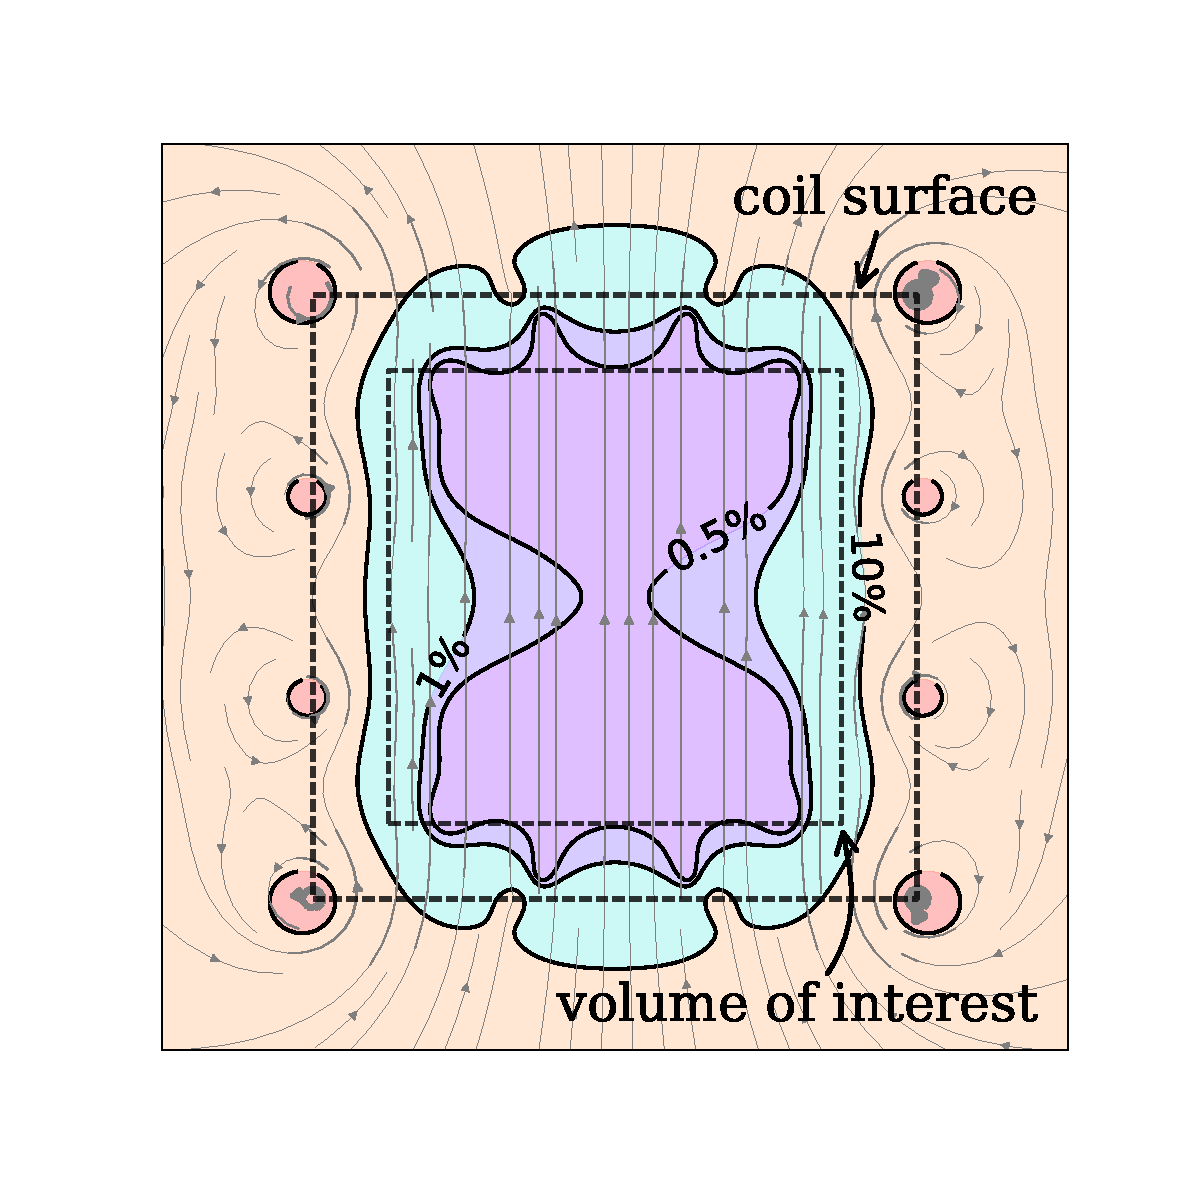
\includegraphics[width=.49\linewidth]{gfx/coils/homogeneous_performance.pdf}}
  \subfloat{\label{fig:homogeneous_performance_b}
    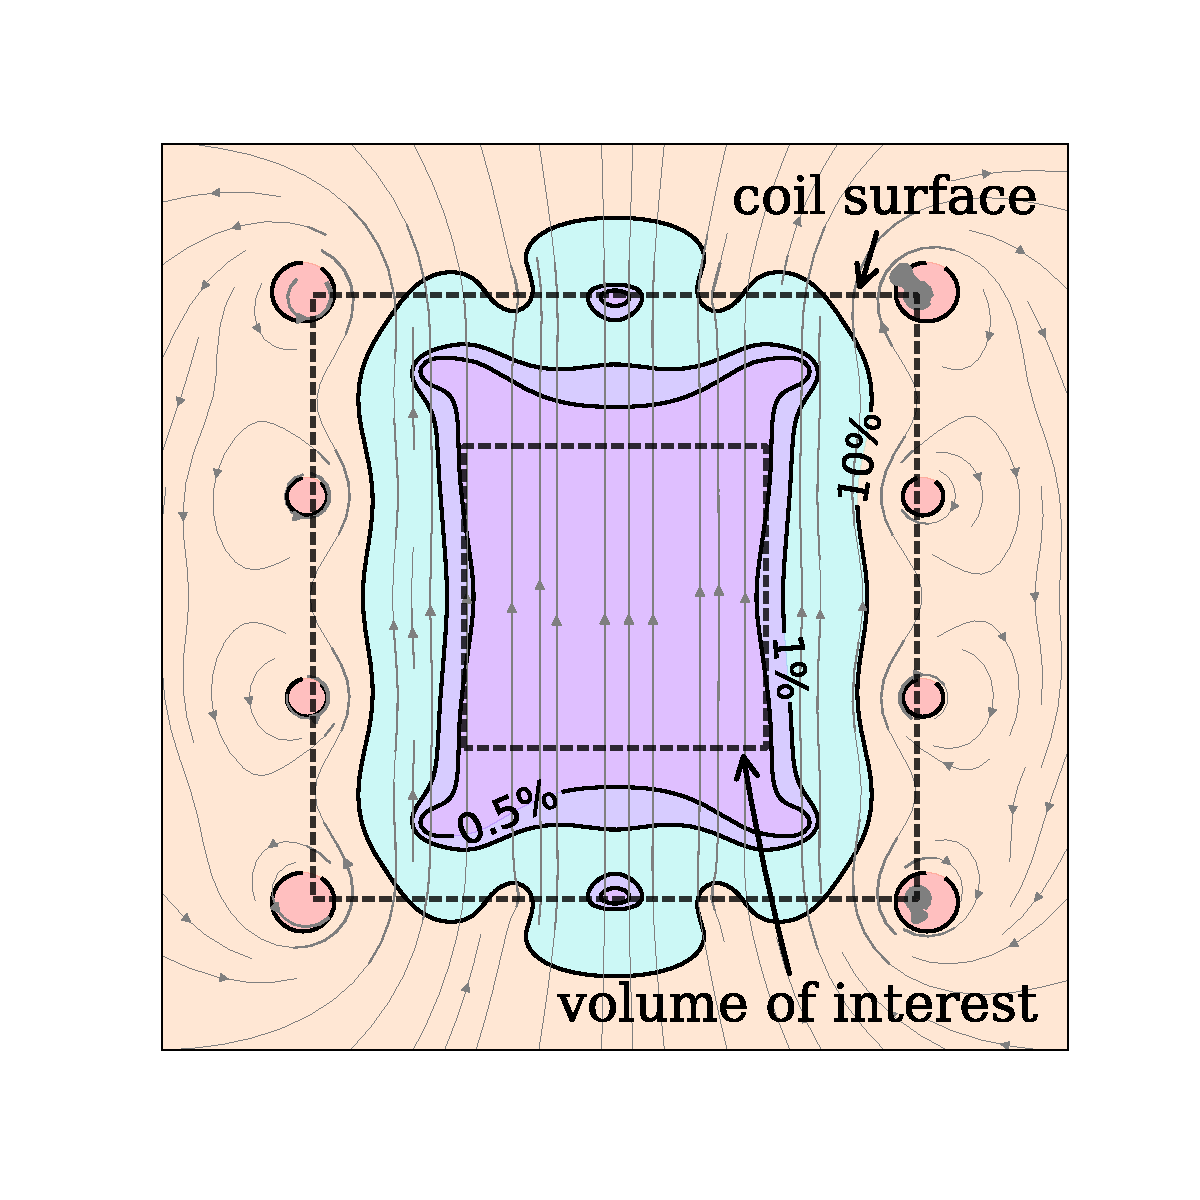
\includegraphics[width=.49\linewidth]{gfx/coils/homogeneous_performance_smaller_volume.pdf}}
  \caption{Magnetic field produced by a coil designed for a homogeneous field, with $N = 6 \times (3 \times 3)$ tiles on a unit cube. The field lines are depicted in grey. Contours show boundaries of \num{0.5}, \num{1} and \SI{10}{\percent} magnitude deviation from an ideal homogeneous field. Horizontal cross sections in the middle-height plane are shown. Two designs are presented. Left-hand side: the volume of interest is a cube with side length \num{0.75} (the individual tile coil currents are depicted in Fig.\,\ref{fig:homogeneous_tiles}), right-hand side: the size of volume of interest is reduced to \num{0.5}.}\label{fig:homogeneous_performance}
\end{figure*}

Let us consider an example of a coil design on a unit cube with the number of tiles $N = 6 \times (3 \times 3)$ (see Fig.\,\ref{fig:homogeneous_tiles}).
As the volume of interest we pick a centered cube with side length \num{0.75} (with a regular mesh of $10 \times 10$ points on each face, a total of $m = 488$ points of interest).
For the sake of simplicity we design a coil for a homogeneous field along an axis of the cube.
The solution of Eq.\,\ref{eq:requirement} directly gives the currents in each tile.
They are graphically depicted in Fig.\,\ref{fig:homogeneous_tiles}.
Note that many currents almost cancel each other out, in particular those along horizontal edges.
The magnetic field produced by the solution is shown on the left-hand side in Fig.\,\ref{fig:homogeneous_performance} as a horizontal cut along the central plane.
Contours show the relative deviation from the homogeneous field.
Inside the volume of interest (dashed line) the design goal of a homogeneous field is reproduced with few per cent accuracy.
The solution, and the contours, depend on the choice of the volume of interest.
In general, the further away the volume of interest is from the coils, the better the accuracy.
If the side length of the volume of interest is decreased to \num{0.5}, the accuracy improves to \SI{1}{\percent}, as shown on the right-hand side in Fig.\,\ref{fig:homogeneous_performance}.
The optimal solution, and thereby the shape of the precision contours change.
The accuracy of the field reproduction can also be improved by increasing the number of tiles.




\section{Simplification of the tile system}
The tile system may find an interesting practical application.
Once independently controllable tiles have been built, it can be used to produce any arbitrary field.
However, building many independently driven coils is a high price to pay for producing only one field.
Additionally, each edge is shared between two tiles, and the effective current is the sum of these.
The currents add either constructively or destructively.
If the given solution is dominated by subtraction of large currents, a lot of power is unnecessarily dissipated in the system.
We find that both problems can be solved by simplifying the tile solution.

\begin{figure*}
  \centering
  \subfloat{\label{fig:coils_dipole_3d_1}
    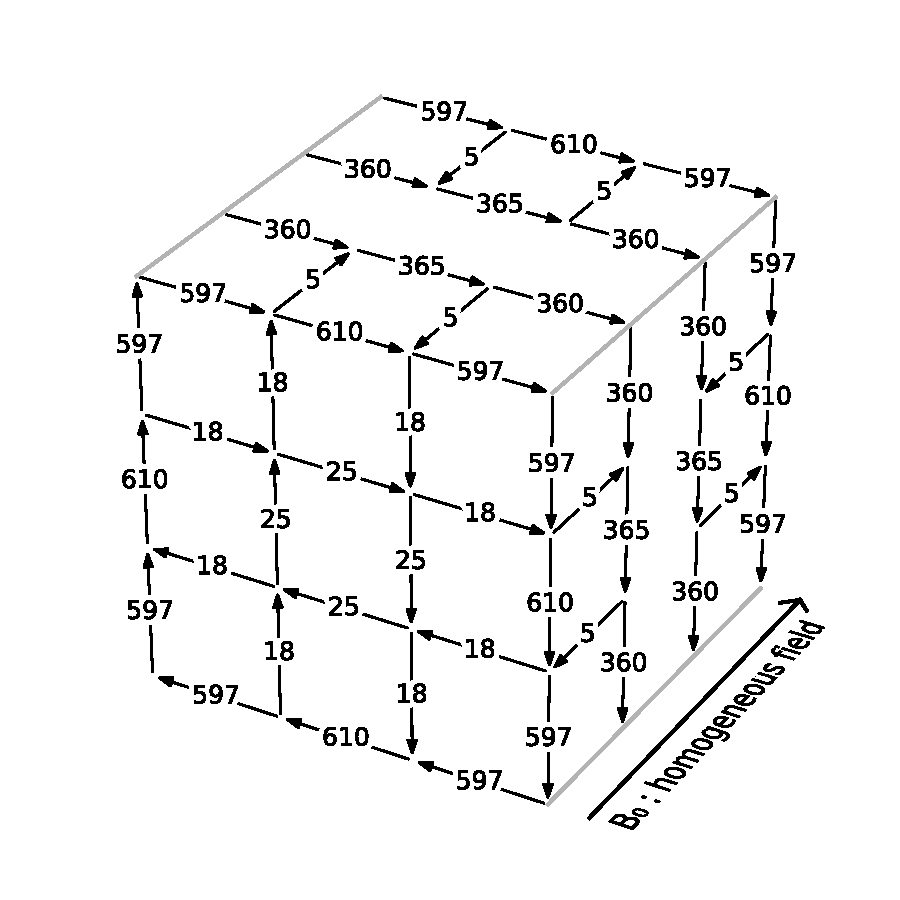
\includegraphics[width=.49\linewidth]{gfx/coils/algorithm_net_1.pdf}}
  \subfloat{\label{fig:coils_dipole_section_0}
    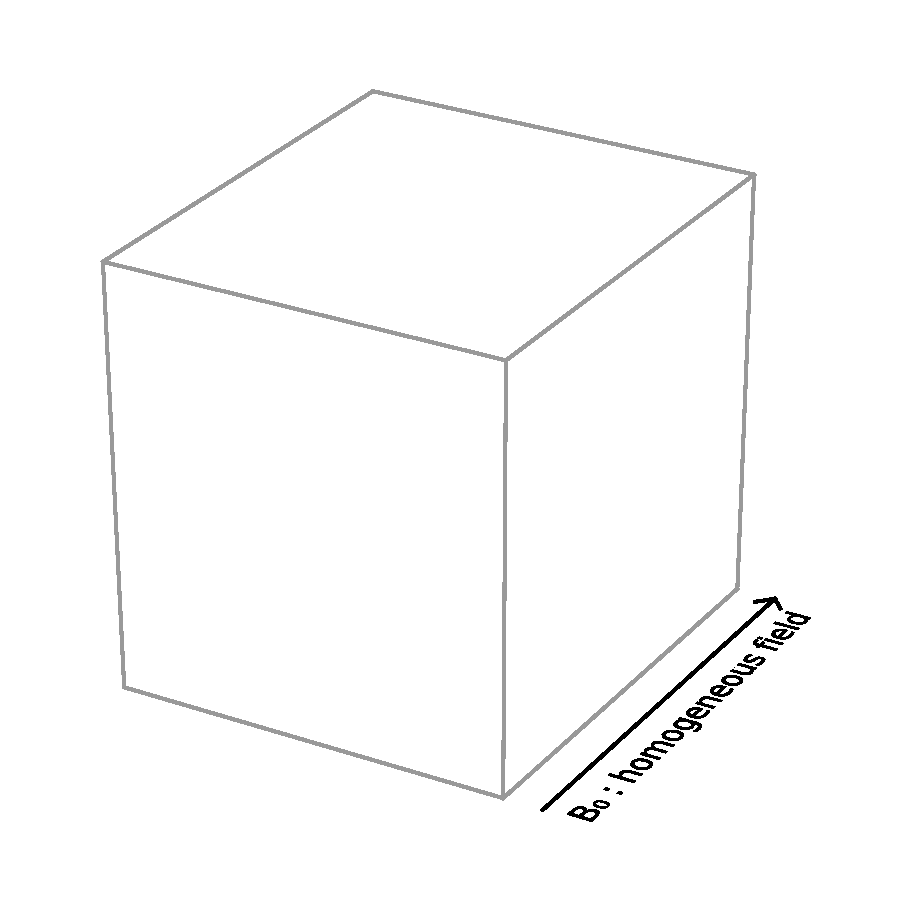
\includegraphics[width=.49\linewidth]{gfx/coils/algorithm_simplified_0.pdf}}
  \\
  \subfloat{\label{fig:coils_dipole_3d_3}
    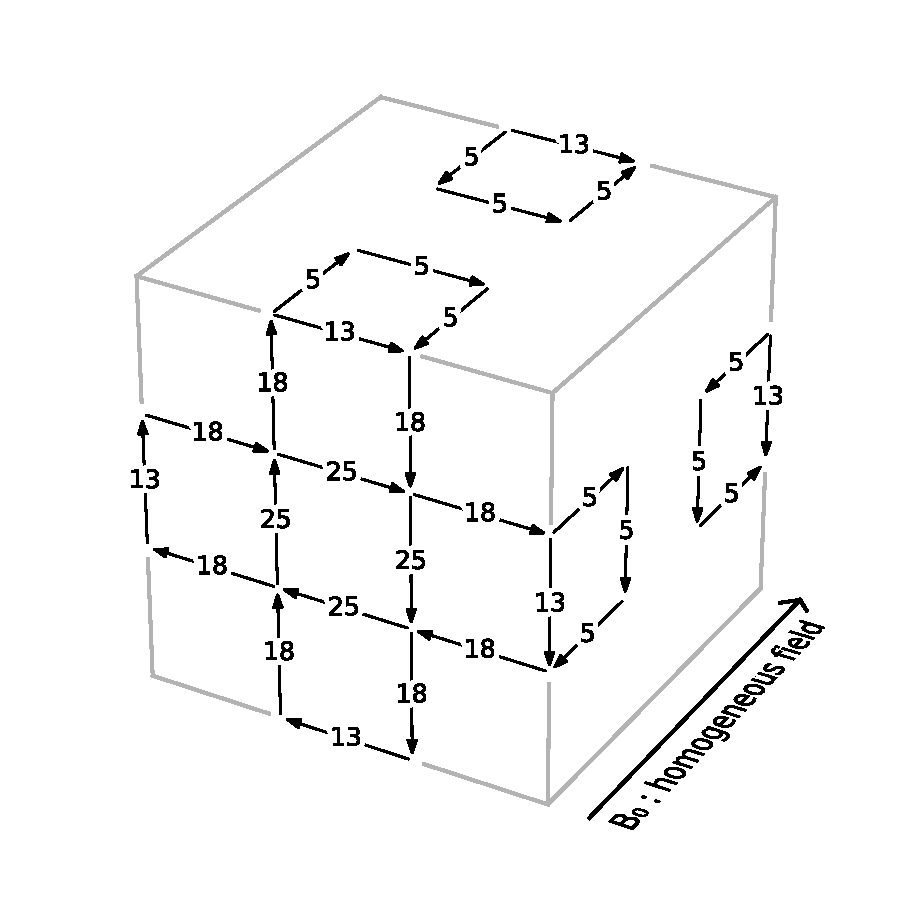
\includegraphics[width=.49\linewidth]{gfx/coils/algorithm_net_3.pdf}}
  \subfloat{\label{fig:coils_dipole_section_2}
    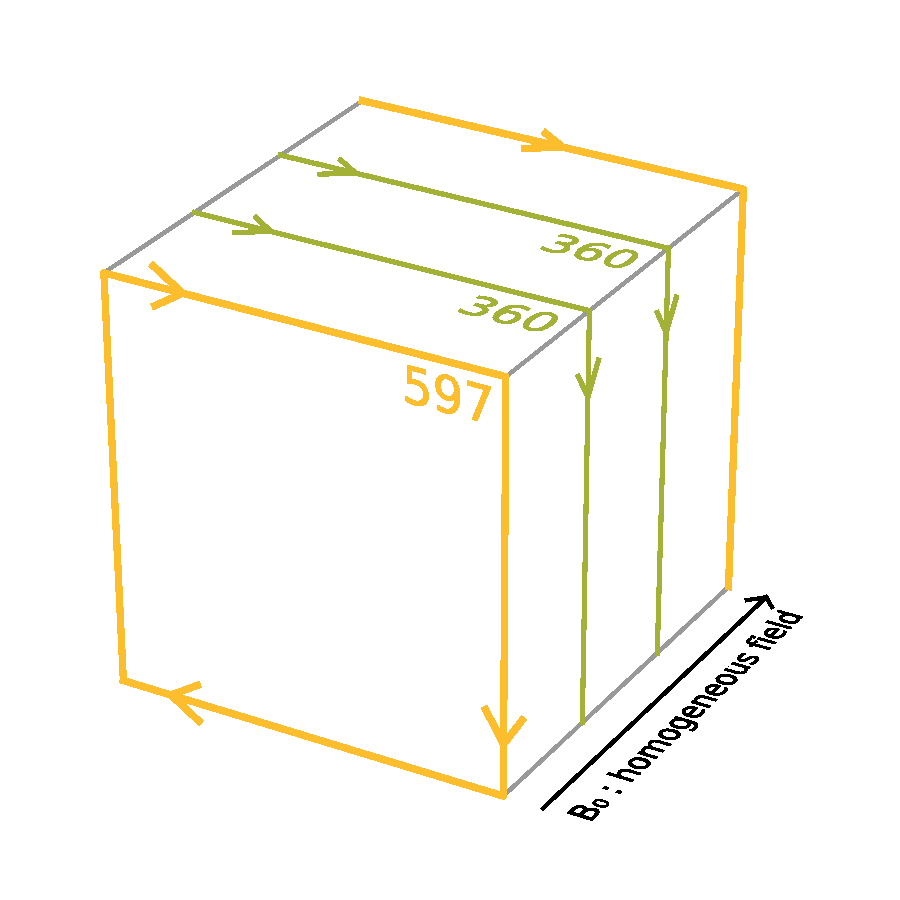
\includegraphics[width=.49\linewidth]{gfx/coils/algorithm_simplified_2.pdf}}
  \\
  \subfloat{\label{fig:coils_dipole_3d_5}
    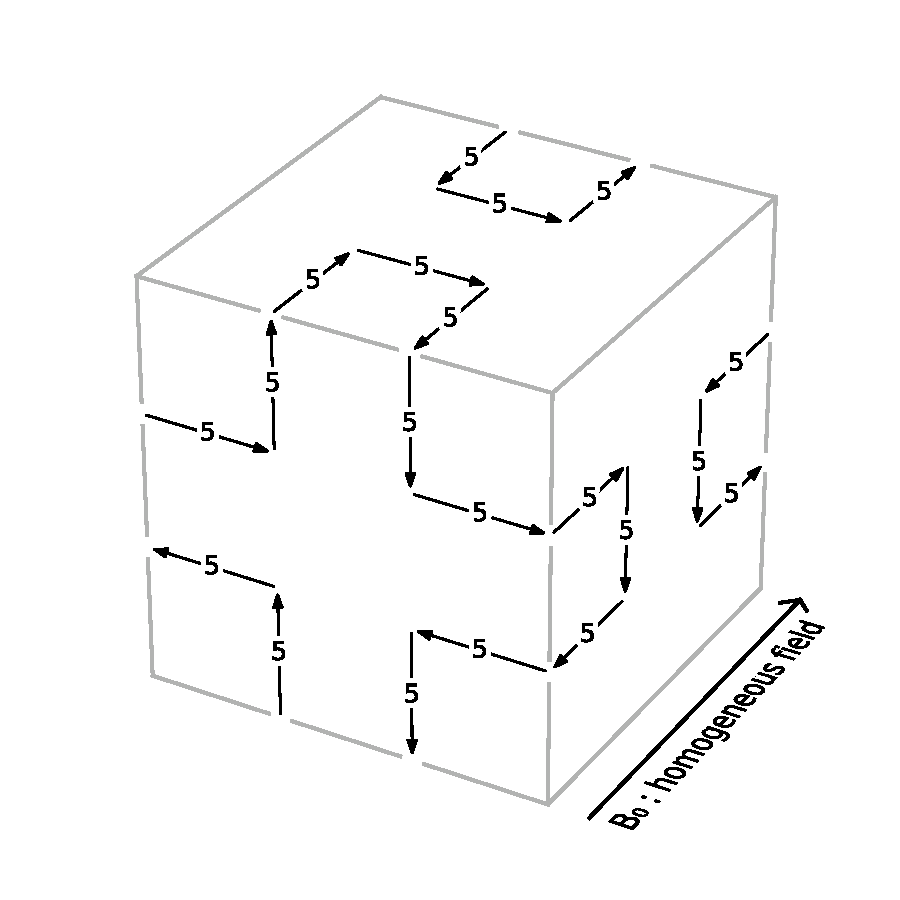
\includegraphics[width=.49\linewidth]{gfx/coils/algorithm_net_5.pdf}}
  \subfloat{\label{fig:coils_dipole_section_4}
    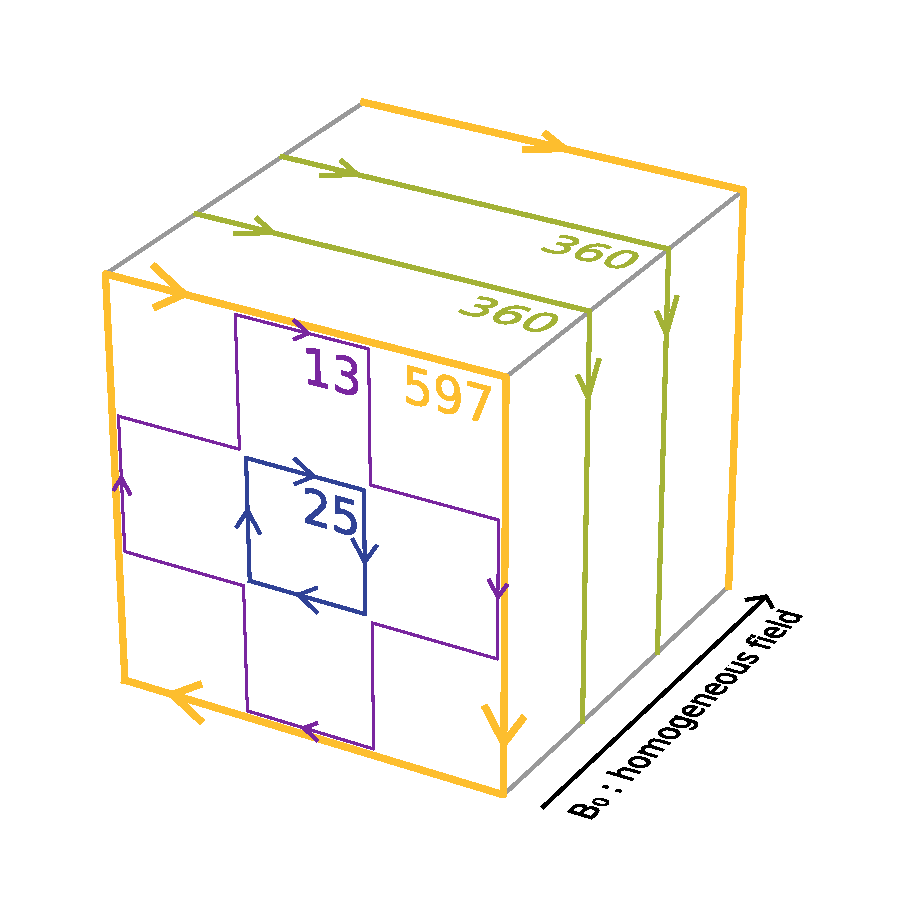
\includegraphics[width=.49\linewidth]{gfx/coils/algorithm_simplified_4.pdf}}
  \caption{Following the algorithm to simplify a coil. The left column shows the net of a current with the total current along edges of tiles. In each iteration the loop with the highest current is found and transferred onto the simplified solution, shown in the right column. We show iterations, from top: zeroth, fourth and eighth.}\label{fig:simplification_algorithm}
\end{figure*}

\begin{figure}
  \centering
  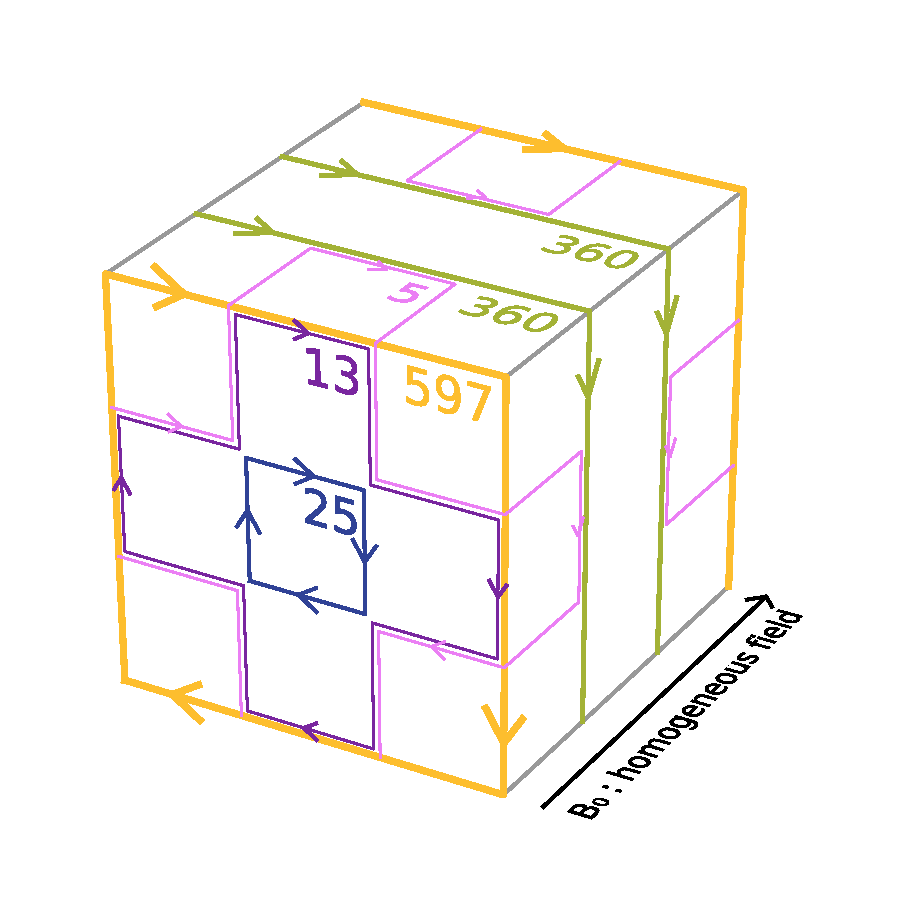
\includegraphics[width=\linewidth]{gfx/coils/algorithm_simplified_5.pdf}
  \caption{The coil designed for a homogeneous field, with $N = 6 \times (3 \times 3)$ tiles (Fig.\,\ref{fig:homogeneous_tiles}), simplified by adding the currents along each edge and decomposing into current loops.}\label{fig:homogeneous_coils}
\end{figure}

One starts by adding the currents of adjacent tiles and assigning the sum to each common edge.
The result is a complicated net of currents (upper left corner of Fig.\,\ref{fig:simplification_algorithm}), with each node fulfilling Kirchhoff's laws. The net can then be decomposed into simple current loops by the following algorithm: First find in the net the loop with the highest current.
In the example it is either of the ``\num{597}'' loops on the front and back faces.
This will be the primary loop in the simplified solution (it can be seen in the middle of the right column in Fig.\,\ref{fig:simplification_algorithm}, together with the next three loops).
Then subtract from the net the current of the primary loop along its edges (the net that remains after subtracting the first four loops is depicted in the middle of the left column in Fig.\,\ref{fig:simplification_algorithm}).
Finally, continue to find the loop with the highest current in the modified net, which will give the next loop and repeat until the current net is empty.
The net remaining after eight loops are found is depicted in the bottom row of Fig.\,\ref{fig:simplification_algorithm}, next to the first eight loops.
The final simplified solution is shown in Fig.\,\ref{fig:homogeneous_coils}.
The currents in the simplified coil system are much smaller, the highest being \num{597} instead of \num{1000} and they always add constructively.
Also, the number of separate loops is decreased from \num{42} to \num{10}.
Still, the total current along each edge of a tile is exactly the same as in the tile configuration.

We conclude here our method of coil design.
The simplified arrangement of coils is optimal, given the grid restriction, for approximating the magnetic field in the volume of interest.
We continue to consider practical aspects, relevant for constructing the designs of the new method.




\section{Practical considerations}
The foremost practical advantage of the new design method is that the coils are constrained to a predefined grid.
This is contrary to other methods of coil design, where the position of the wires is the output of the procedure~\cite{Turner1993, Beidler1990}. This may prove useful in applications with spatial constraints.
Typically, coils need to be incorporated into a setup in which other components penetrate the surface on which the wires are laid.
With the new method it is possible to simply define the grid so that no collisions occur.
Although the simple examples presented before used regular grids, we have not used symmetries to solve the problem.
When many coils are designed and built, for instance to produce homogeneous magnetic fields in each of the three dimensions, they can all share the same grid.
The grid can, for example, be constructed out of cable channels into which the wires are laid.

A limitation associated with the finite size of the channels is the strength of the magnetic field that can be created, which for a given available power is limited by the thickness of the wire.
At the same time, the finite size of the cable channels can be neglected in the calculations, only as long as it is small compared to the distance between the coils and the volume of interest.
Using an enameled wire, rather than the standard, PVC-insulated cable, we can reduce the overall thickness.

In order to produce the desired field, one still needs a system of several coils, even in the simplified solution.
The more complicated the goal field, and the more tiles, the greater the number of currents across the individual loops is required, which quickly becomes impractical.
There are several ways to tackle the problem.

The first way is to use only one current and adjust the magnitude by varying the number of windings.
In the example when one decides for \num{60} windings as the maximum, the nominal current that would flow through the wire is $\mathrm{round}(597 / 60) = 10$.
 \num{597}, \num{360}, \num{25}, \num{13} and \num{5} would be created with \num{60}, \num{36}, \num{3}, \num{1} and \num{1} windings, respectively.
A discretisation error of $10 / 597 = \SI{1.7}{\percent}$ is of the same order as the accuracy of the solution in representing the field (see Fig.\,\ref{fig:homogeneous_performance}).
For more precise designs the numbers of windings increase, which is more difficult to construct and causes the coils to have larger inductances.

A second way is to use a current divider.
This connects the different loops in parallel, each with an appropriately chosen resistance in series.
This way the ratios between the currents in each loop can be tuned precisely.
However, a practical realization will most likely involve routing all loops out of the system where the current divider is installed.
For more complicated coil systems with tens of different currents this may be impractical.

Yet another way is to split the loops into decades of currents.
In the coil we use as an example, the currents \num{597}, \num{360}, \num{13}, \num{7}, \num{5} (in arbitrary units) may be constructed from a set of wires with three relative currents of \num{100}, \num{10} and \num{1}:
\marginpar{A base different than 10 can be used, too.}
\begin{align*}
  597 & = 5 \times 100 + 9 \times 10 + 7 \times 1 \\
  360 & = 3 \times 100 + 6 \times 10 + 0 \times 1 \\
  13 & = 0 \times 100 + 1 \times 10 + 3 \times 1 \\
  7 & = 0 \times 100 + 0 \times 10 + 7 \times 1 \\
  5 & = 0 \times 100 + 0 \times 10 + 5 \times 1 \ .
\end{align*}
Using this method, a reproduction accuracy better than \SI{1}{\percent} can be reached with only three different currents to control, even for complicated designs.
Those can be either separately controlled or split with a current divider.

No claim is made as to the superiority of one of the three above solutions over the other two.
The best solution is up to the particular application for which it is required.




\section{Application to active magnetic field shielding}
Using the method presented here to design coils of an active magnetic shield  offers improvements in two areas.
Firstly, the size of the coils could be decreased, or the size of the experimental set-up increased, without loss of performance.
Better homogeneity in a given volume can always be achieved by choosing a denser grid.
Given the tight spatial constraints this was a crucial development for the design of the n2EDM active shield.

\begin{table}
  \centering
  \begin{tabular}{c|ccc}
    n & $\mathbf{P}_n^x(\mathbf{r})$ & $P_n^y(\mathbf{r})$ & $P_n^y(\mathbf{r})$ \\ \midrule
    1 & 1 & 0 & 0 \\
    2 & 0 & 1 & 0 \\
    3 & 0 & 0 & 1 \\
    \midrule
    4 & $x$ &  0  & $-z$ \\
    5 & $y$ & $x$ &   0  \\
    6 &  0  & $y$ & $-z$ \\
    7 & $z$ &  0  & $ x$ \\
    8 &  0  & $z$ & $-y$ \\
  \end{tabular}
  \caption{Cartesian harmonic polynomials. Further terms can be found for example in Ref.\,\cite{Franke2013}.}\label{tab:coils_cartesian_harmonics}
\end{table}

Secondly, the method allows to construct a coil for any field.
In particular, one may choose to construct coils that produce fields orthogonal to one another. 
% (as $\mathbb{R}^3 \rightarrow \mathbb{R}^3$ functions).
This makes an active shielding system significantly easier to control~\cite{MRM:MRM1910010107} and avoids potential problems in the high condition number due to very-high-order fields produced by pathological combinations of coils (recall the discussion in Sec.\,\ref{sec:nedm_sfc_matrix}).
One of the possible orthogonal decompositions of the field is into \emph{cartesian harmonic polynomials}~\cite{Franke2013}:
\begin{equation}
  \mathbf{B}(\mathbf{r}) = \sum_{n}\,H_n \mathbf{P}_n(\mathbf{r}) \ ,
\end{equation}
where $H_n$ are the expansion coefficients and $\mathbf{P}_n(\mathbf{r})$ are the cartesian harmonic polynomials, the first eight of which are listed in Table~\ref{tab:coils_cartesian_harmonics}.
Each term satisfies Maxwell's equations by itself.
The first three terms are homogeneous fields, the next five are the five independent linear gradients.
Further terms correspond to higher-order gradients.

\begin{figure*}
  \centering
  \subfloat{\label{fig:coils_dipole_3d}
    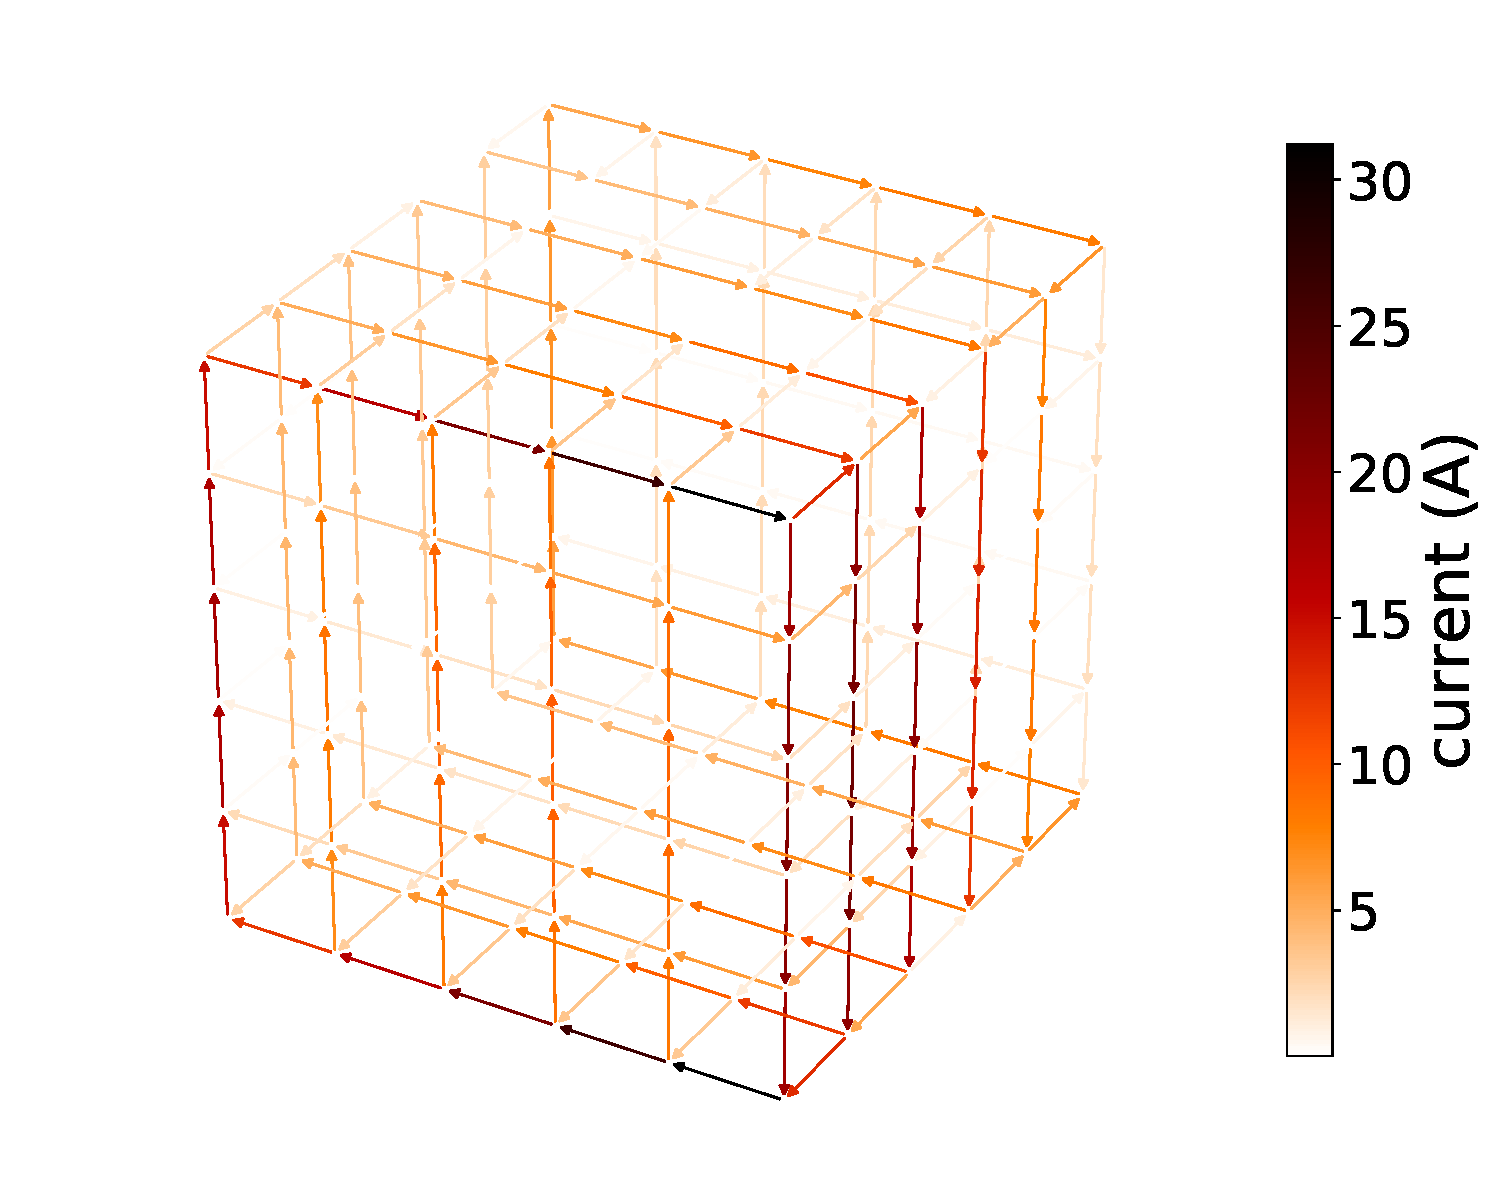
\includegraphics[width=.39\linewidth]{gfx/coils/coil_dipole.pdf}}
  \subfloat{\label{fig:coils_dipole_section}
    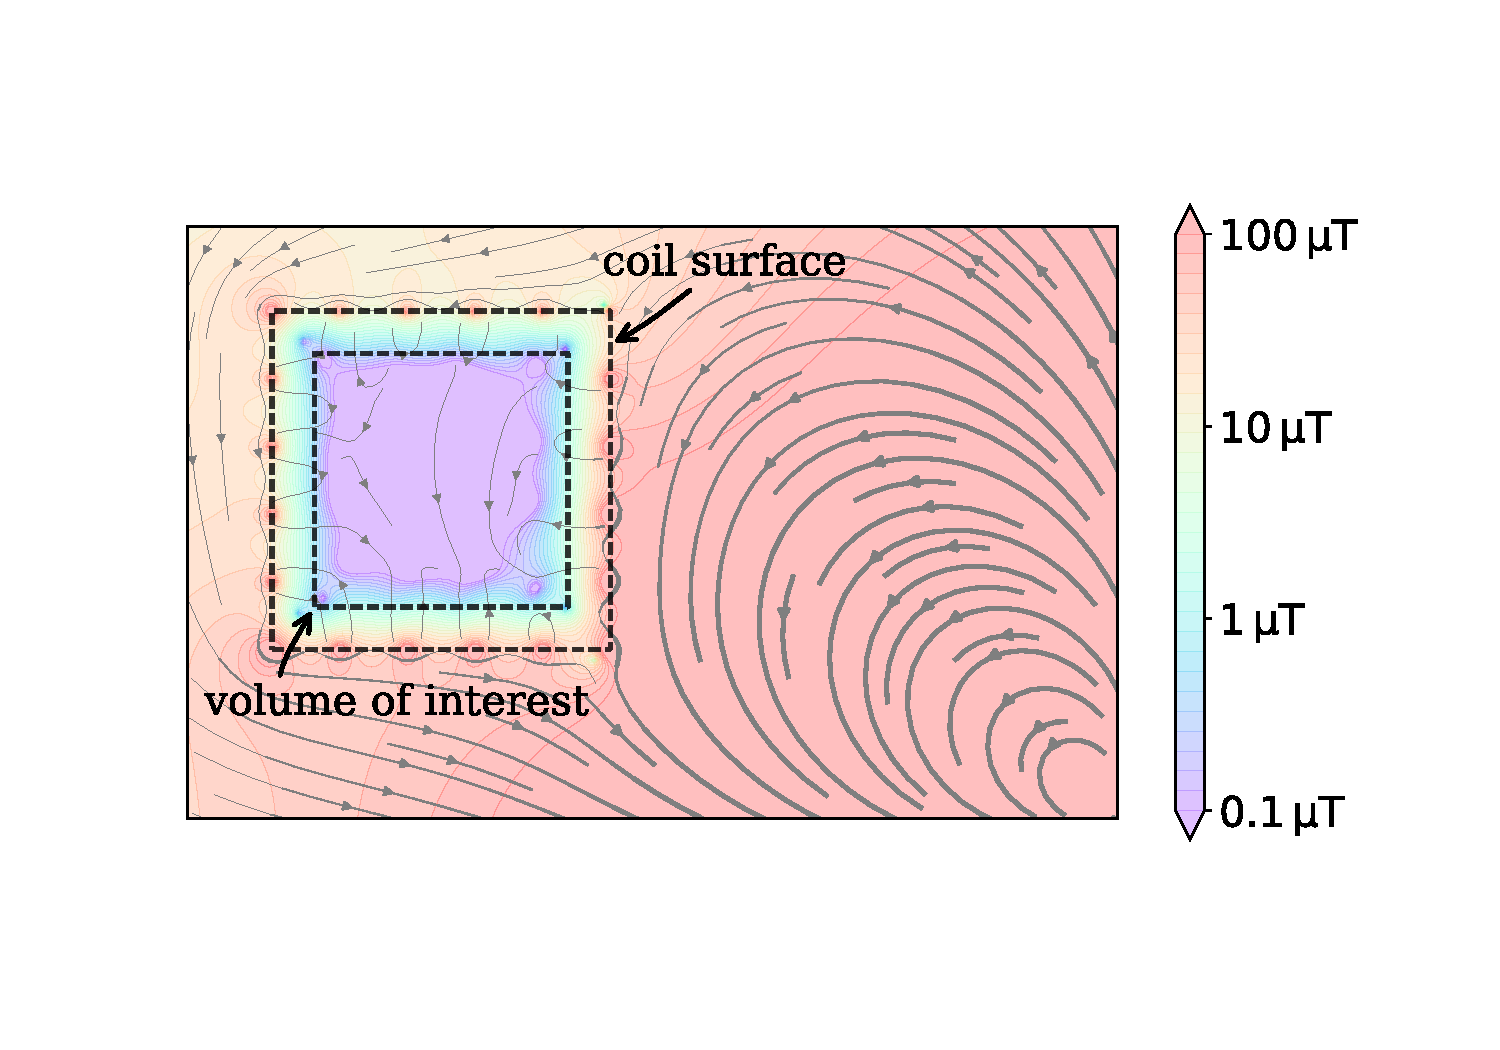
\includegraphics[width=.59\linewidth]{gfx/coils/coil_dipole_section_with_dipole.pdf}}
  \caption{A coil designed on a unit cube with $5 \times 5$ tiles per face to shield against a dipole disturbance. The dipole is located, relative to the center of the unit cube, two units to the right and one unit to the front. It is located in the middle height of the cube. The volume of interest has a side length of \num{0.75}. On the left-hand side the total current along each edge of the dipole compensation coil is depicted. On the right-hand side the magnetic field is shown. The magnetic field lines are shown in grey, the volume of interest and the coil surface with dashed lines. The colors depict the magnitude of the magnetic field (capped at \num{0.1} and \SI{100}{\micro\tesla}). A horizontal cross section in the middle height is shown. The dipole source is located in the lower right corner of the plot and points parallel to the plane of the plot. The magnitude of the field in the volume of interest is reduced from tens of microteslas down to below one.}\label{fig:showcase}
\end{figure*}

Additionally, one can consider constructing dedicated coils to counteract a particular known disturbance.
In Fig.\,\ref{fig:showcase} a showcase design with $N = 6 \times (5 \times 5) = 150$ tiles for compensating a nearby dipole source is presented.

Lastly, the method's unique property of designing coils on a predefined grid makes a large-scale construction particularly simple.
It makes the coil array easily incorporated into existing structures by defining the grid in a conflict-free way.




\section*{Coil design -- conclusion}
Coil design is a complicated and very technical problem, especially when high accuracy is required. This work presents a method that is simple in terms of both underlying maths and computational effort.
The design method could find its niche in practical applications, where spatial constraints play a significant role and a percent level in accuracy of the produced field is acceptable.
The method has particular advantages when used to design coils of an active magnetic field compensation system.
In the next chapter, its application to construction of a compensation system at ETH Zürich is described.

The software implementation of the coil design, including examples, has been published as an open-source and can be accessed in Ref.\,~\cite{Coilsjlcode}.
